% SVN info for this file
\svnidlong
{$HeadURL$}
{$LastChangedDate$}
{$LastChangedRevision$}
{$LastChangedBy$}

\chapter{Il campo magnetico}
\labelChapter{campoMagnetico}

\begin{introduction}
	``Il magnetismo è la forza che fa sì che certi oggetti siano attratti ai frigoriferi.''
	\begin{flushright}
		\textscsl{Dave Barry}, poco prima di essere bocciato al secondo appello.
	\end{flushright}
\end{introduction}
\lettrine[findent=1pt, nindent=0pt]{R}{icordate il} problema fondamentale dell'elettrodinamica classica? Date delle sorgenti di carica, vogliamo sapere la forza esercitata su una carica di prova. Nella prima parte di questo Manualozzo\texttrademark\ ci siamo dedicati quasi esclusivamente a cariche statiche, ossia all'elettrostatica - certo, il \autoref{chap:correnteElettrica} riguardava cariche in moto, ma lì ci siamo limitati di fatto allo studio dell'elettrotecnica, senza aver visto come tale moto di cariche influenzi altre cariche. Tuttavia, per capire ciò, dobbiamo parlare di \textbf{magnetismo}.

In questo Capitolo inizieremo il nostro viaggio nella \textbf{magnetostatica}, ossia nei fenomeni magnetici non dipendenti dal tempo, con un excursus storico dello studio del magnetismi; utilizzando il formalismo dei campi vettoriali, parleremo di come cambia la \textbf{legge di Gauss} per il campo magnetico. Successivamente, vedremo due esperimenti fondamentali  di inizio '800 svolti da \textbf{Oersted} e da \textbf{Ampère}, che ci faranno capire alcune stranezze del campo magnetico.

Nella seconda parte inizieremo a collegare formalmente tutte queste informazioni introducendo la \textbf{forza di Lorentz}; da questa legge empirica dimostreremo poi la \textbf{seconda legge di Laplace} e ne vedremo un'applicazione meccanica parlando di una spira libera di ruotare immersa in un campo magnetico.
\section{I primi studi sul magnetismo}
Come già detto nel \autoref{chap:leggediCoulomb}, il termine magnetismo deriva da \textit{magnētis lithos}, ``pietra di Magnesia'' in greco: sull'isola egea di Magnesia erano diffuse rocce di \textit{magnetite}, un minerale ferroso che in certi casi è capace di attrarre piccoli pezzetti di ferro - che a loro volta diventavano magnetici.
Il fatto che la magnetite può attrarre il ferro fu osservato non solo in Grecia, ma in diverse aree geografiche: in India, ad esempio, la magnetite veniva usata per rimuovere le frecce infilzate nel corpo di una persona.
\paragraph{La bussola}
Un altro luogo fondamentale per la storia del magnetismo fu la Cina. Durante la \textit{dinastia Han} (202 a.C – 220 d.C.) furono inventate le prime (rudimentali) \textbf{bussole}\index{bussola}: esse consistevano in un ago di \textit{magnetite naturalmente magnetica} che, se lasciato libero di ruotare, indicava sempre verso una particolare direzione terrestre: il \textit{nord} o il \textit{sud}.

Tuttavia, i primi utilizzi della bussola erano di natura \textit{divinatoria}: le proprietà ``indirizzanti'' di tale strumenti furono usate per trovare il luogo dove costruire case, piantare le coltivazioni e cercare gemme rare.\footnote{\textbf{Shen Kuo}, scienziato della dinastia Song (960 – 1279) descrisse dettagliatamente come gli esperti di \textit{feng shui}, un arte divinatoria geomantica, magnetizzavano la punta di ago con magnetite magnetica e lo appendevano con un singolo filo di seta per mezzo di un pochino di cera al centro dell'ago. Shen Kuo riportò inoltre che l'ago preparato in questo modo ogni tanto puntava verso sud, ogni tanto verso nord.} Per l'utilizzo nella \textit{navigazione} bisogna aspettare diversi secoli: la prima fonte certa a riguardo è di Zhu Yu, datata tra il 1111 e il 1117. Qualche decennio più tardi la bussola da navigazione si era diffusa anche in Europa e nel mondo arabo.

L'invenzione della bussola permise di osservare ulteriori proprietà dei magneti. Ad esempio, si notò che avvicinando una bussola ad un oggetto magnetico essa \textit{non} indicava più la direzione nord della terra, bensì puntava \textit{verso l'oggetto}.\\
In particolare, il ``polo nord della bussola'' - ossia il capo dell'ago che normalmente punta verso il nord terrestre - puntava verso una parte specifica dell'oggetto, mentre era respinto dal resto.\\
\begin{minipage}{0.79\textwidth}
D'altro canto, il ``polo sud della bussola'' - ossia il capo dell'ago che normalmente punta verso il sud terrestre  - funzionava al contrario: era attratto dalla parte che \textit{respingeva} il polo nord della bussola e, viceversa, era \textit{respinto} dalla parte che attraeva il polo nord della bussola.
In altre parole, si dedusse che come i \textit{poli terrestri} attraevano la bussola nella direzione nord-sud, anche i magneti dovevano avere sempre due \textbf{poli magnetici}\index{polo!magnetico}, a cui la bussola punta se vicina al magnete.
\end{minipage}\hspace{5pt}
\begin{minipage}{0.2\textwidth}
\begin{center}
	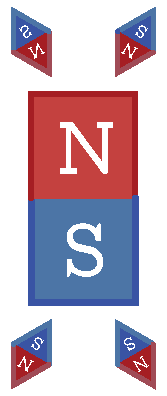
\includegraphics[width=0.45\textwidth]{images/chp7/chp7magnetebussola.pdf}
\end{center}
\end{minipage}
I poli dei magneti sono quindi tradizionalmente indicati come \textit{nord} e \textit{sud}, in analogia con quelli terrestri.
\begin{digressionwt}[\textit{Una montagna da Watussi.} Una breve storia sulla bussola e i poli magnetici terrestri nell'Età delle Grandi Scoperte]
	Sebbene i marinai utilizzassero le bussole da diversi secoli, molti studiosi tra la fine del Medioevo e l'inizio dell'Età Moderna si chiesero \textit{come mai} le bussole, in condizioni normali, puntavano verso una \textit{direzione cardinale} come il nord o il sud.\newline~\\
	Con gli occhi del \textit{fisico moderno} sappiamo perché e lo approfondiremo in questi capitoli: l'ago magnetico della bussola si allinea \textit{parallelamente alle linee di forza} del campo magnetico terrestre - anche se non necessariamente punta ad uno dei due poli.\\
	Tuttavia, per molti secoli il funzionamento di tale strumento rimase particolarmente oscuro - come del resto gran parte del magnetismo. Per un filosofo naturale il concetto di \textit{campo vettoriale} era semplicemente ignoto, e la miglior ipotesi dell'epoca era che la fonte dell'attrazione magnetica notata dalle bussole dovesse essere sempre e comunque \textit{localizzata} in un particolare punto.\newline~\\
	Inizialmente, si suppose che la sorgente attrattiva fosse in cielo, ad esempio la Stella Polare o i poli celesti. Tale ipotesi fu presto sostituita da un'alternativa ``terrena'', come una roccia o una montagna. Nelle cartine europee del XVI secolo si possono spesso notare tali \textit{montagne magnetiche}, come nelle mappe di \textbf{Gerardo Mercatore} (1512 - 1594).
	Il cartografo fiammingo era solito piazzarla in posizione \textit{arbitraria}, ma nel 1546 pensò bene di diventare un cartografo rigoroso e di trovare il luogo in cui era situata sulla base di precisi osservazioni della bussola in varie zone europee: chiaramente, se tracciassimo una linea immaginaria diretta come l'ago della bussola, si dovrebbe trovare un unico punto di incontro corrispondente al luogo della \textit{montagna magnetica}!
	
	Eppure, tale tentativo andò male: non c'era un unico punto di incontro di queste linee. Amareggiato ma non scoraggiato, fece ulteriori misurazioni per \textit{oltre due decenni}, senza successo: ogni volta otteneva due stime completamente contraddittorie per il potenziale polo. Solo poco prima della sua morte Mercatore decise di tagliare la testa al toro e di piazzare due montagne e due poli... ma tali poli \textit{non coincidevano} con le fantomatiche montagne!\newline~\\
	Nella cartina ``\textit{Septentrionalium Terrarum descriptio. Per Gerardum Mercatorem Cum Privilegio}'',  pubblicata postuma, possiamo notare due montagne: una ``\textit{rupes nigra et altissima}'' (\textit{montagna nera e altissima}) posta nei pressi del \textit{Polo Nord geografico}, non era magnetica, mentre l'altra sì e corrispondeva al ``\textit{Polus magnetis respectu insularum capitis Viridis}'' (\textit{polo magnetico rispetto all'arcipelago di Capo Verde}).\\
	Il secondo polo magnetico, ``\textit{Polus magnetis respectu Corui insule}'' (\textit{polo magnetico rispetto alle isole del Corvo\footnote{Probabilmente da intendersi come le isole del gruppo occidentali dell'\textit{arcipelago delle Azzorre}, tra cui l'omonima \textit{isola del Corvo}.}}) lo pose invece in mezzo al \textit{mar Artico}, tra la \textit{Siberia} e la \textit{California}.
	\begin{center}
			\setlength{\fboxsep}{0pt}
			\setlength{\fboxrule}{1pt}
			\fbox{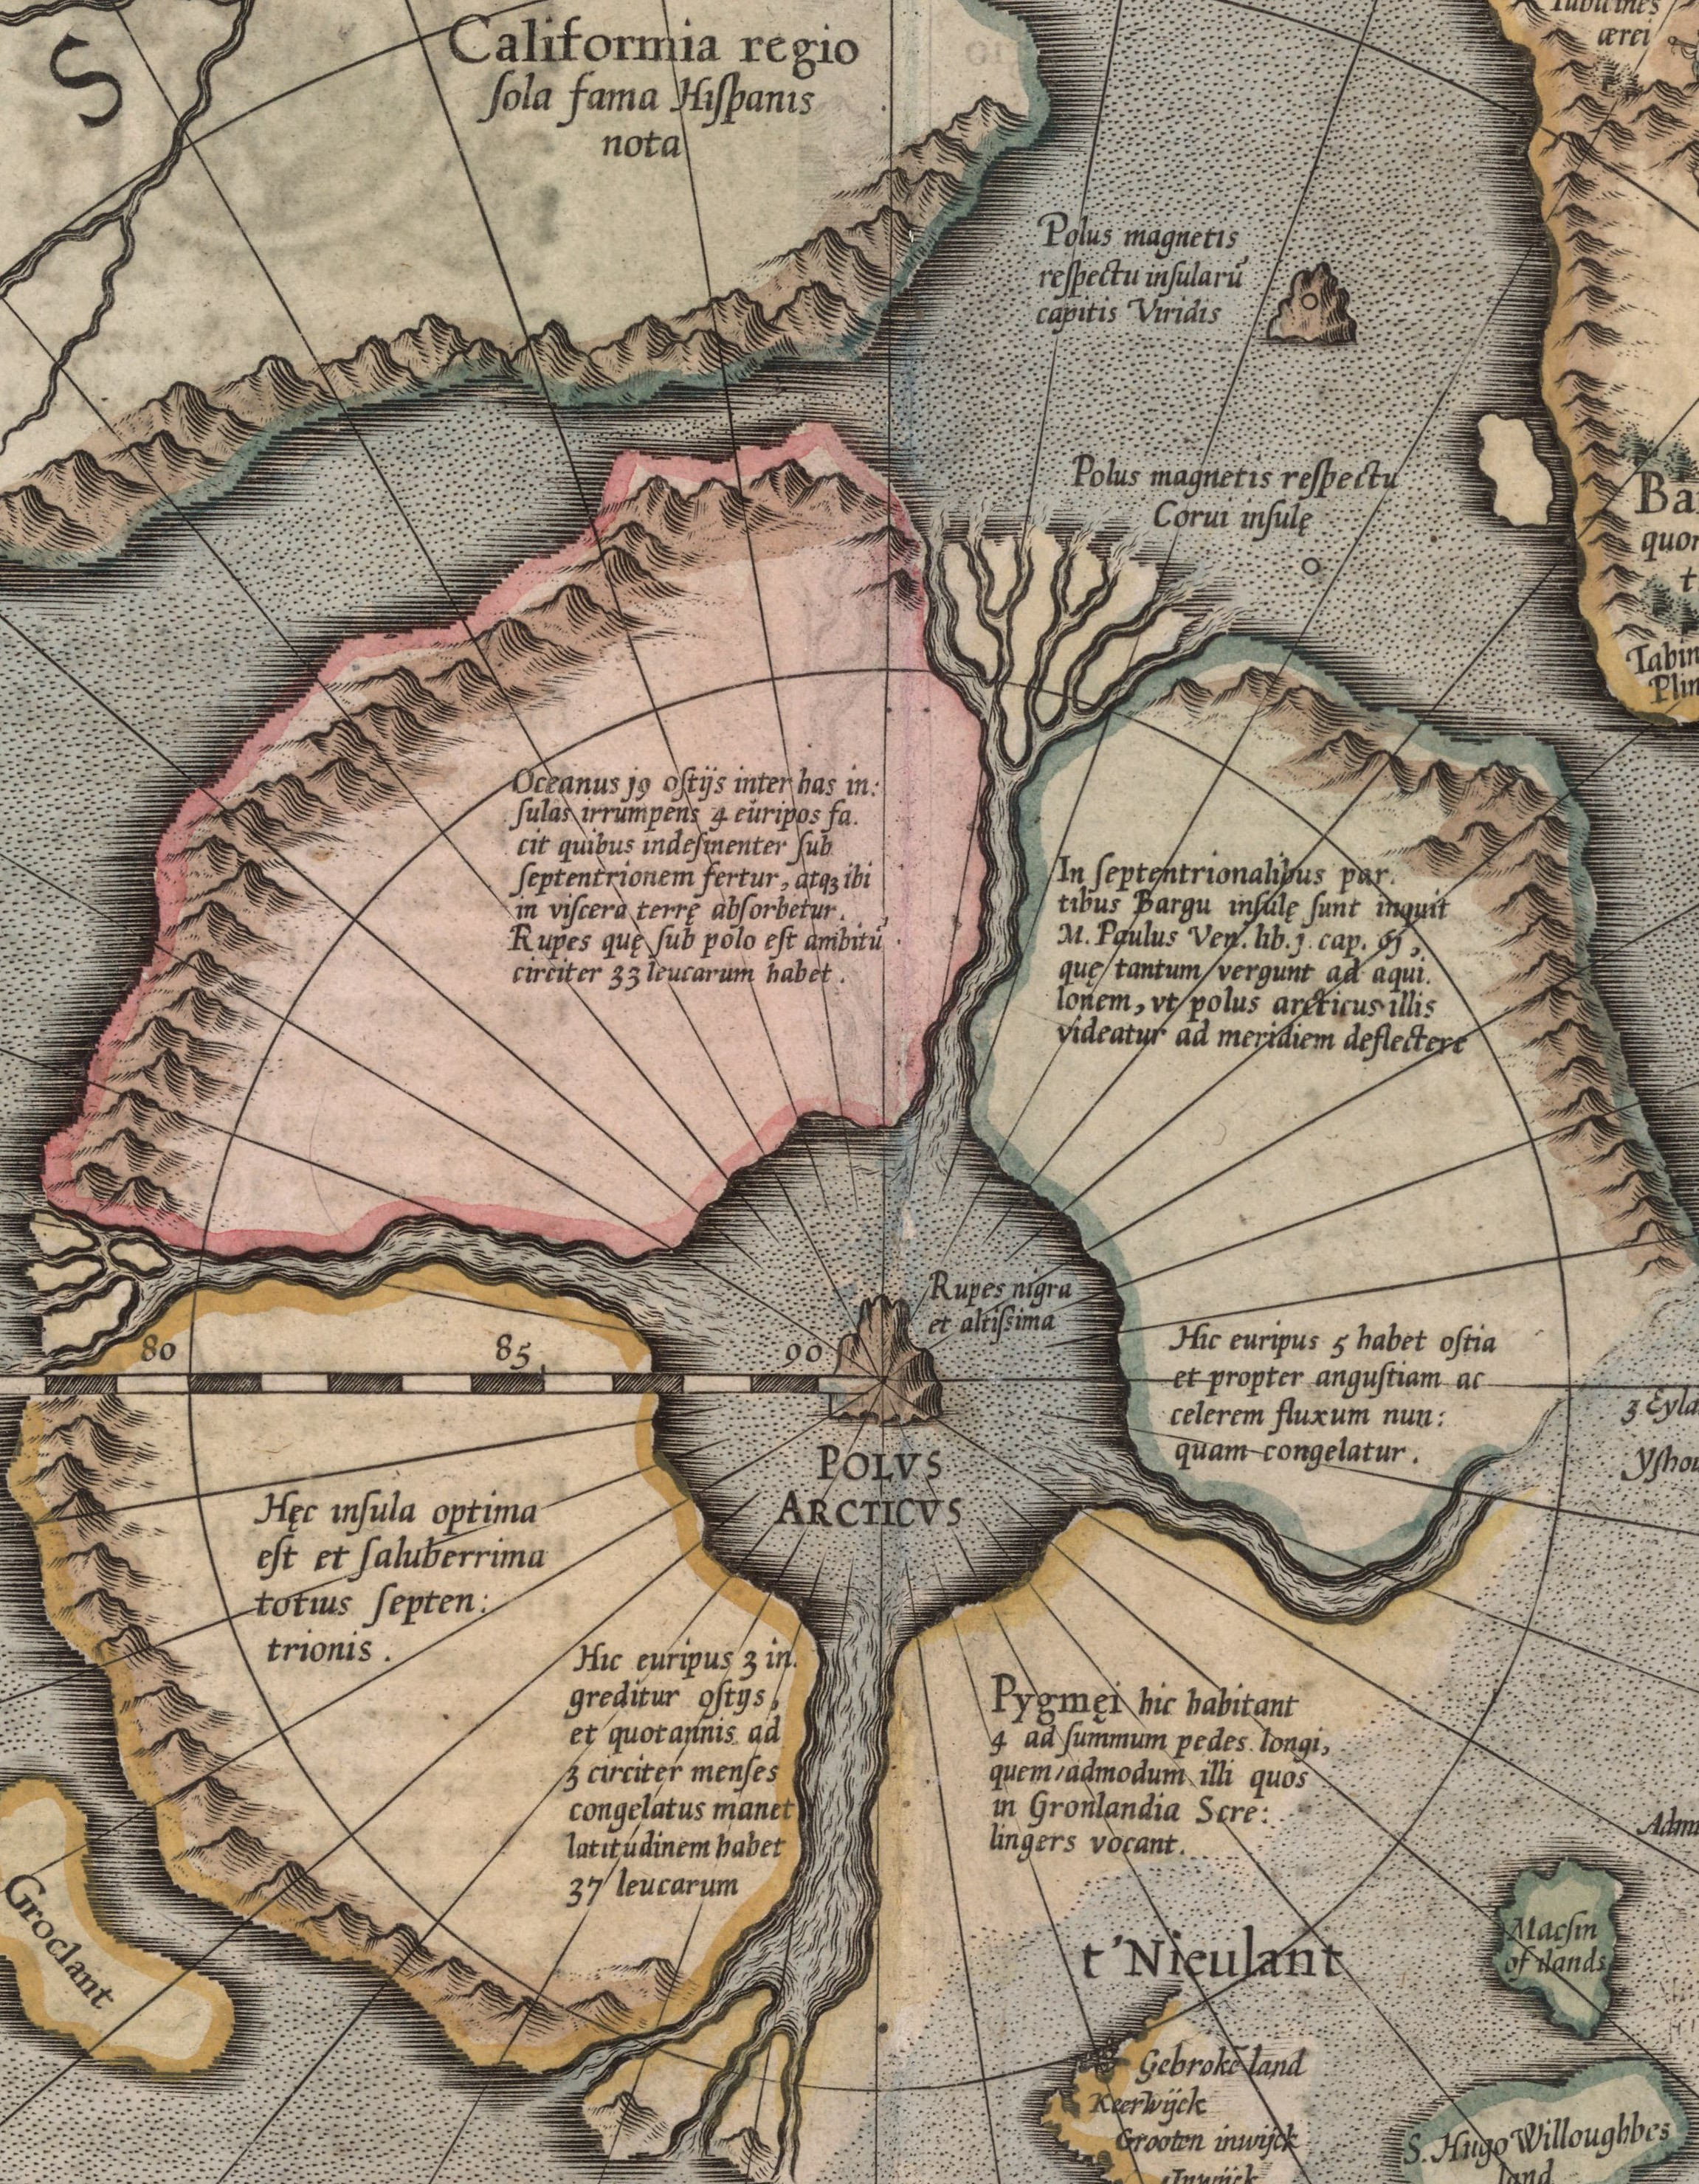
\includegraphics[width=0.75\textwidth]{images/mercator.jpg}}
	\end{center}
\begin{center}
	{\scriptsize Sebbene noto per l'omononima proiezione cartografica, Mercatore fu anche il primo cartografo a creare una mappa dell'Artico, di cui riportiamo un particolare di una versione a colori del 1623. Oltre alle due \textit{montagne} e ai due \textit{poli}, si notano il Polo Nord \textit{quadripartito} in isole separate da fiumi, di cui una abitata da \textit{pigmei}, e la \textit{California spagnola}, erroneamente posta alle stesse latitudini della \textit{Kamchatka}.}% mercatore si inventa un po' le robe, ragazzi
\end{center}
	Fu solo nel 1600 che \textbf{William Gilbert} (1544 - 1603) popolarizzò, nel suo ``\textit{De Magnete}'', un approccio sperimentale per dedurre che \textit{la Terra stessa} fosse un magnete. Con questo sperimento, Gilbert provò che il motivo per cui le bussole erano attratte dai poli terrestri è perché in loro prossimità c'erano dei \textit{poli magnetici} da cui, per dirla in termini moderni, uscivano e entravano le linee di flusso a cui le bussole si allineano. Successivamente, si notò anche che il campo magnetico terrestre non è costante nel tempo, ma varia e con esso variano anche le posizioni dei poli magnetici, da cui spiegato il perché il polo sembrava non essere univoco.\\
	La scelta di Mercatore di porre un polo magnetico senza una montagna ad esso associato - probabilmente dettata dalla disperazione dopo anni e anni di misurazioni fallimentari - in fondo non fu così peregrina: dopotutto, non c'era alcun bisogno di una montagna alta e di colore per far funzionare la bussola.
\end{digressionwt}
\paragraph{La forza magnetica e l'assenza dei monopoli}
Per avere degli studi quantitativi dei fenomeni magnetici bisognerà aspettare il francese \textbf{Charles Coulomb} (1736-1806), il quale osservò che tra due magneti si presentava un \textit{forza}, di diversa natura a seconda di come erano orientati i magneti:
\begin{itemize}
	\item Si aveva una \textit{attrattiva} se si avvicinavano tra di loro i poli opposti (nord - sud).
	\item Si aveva invece una forza \textit{repulsiva} se si avvicinavano tra di loro due poli uguali (nord - nord o sud - sud).
\end{itemize}
Tale forza era direttamente proporzionale al prodotto delle ``intensità'' dei magneti e inversamente proporzionale al quadrato della distanza $r$ tra i due magneti, mentre sembrava - in modo analogo alla \textit{forza elettrica di Coulomb} che era diretta da una carica all'altra - diretta da un polo all'altro.

La situazione potrebbe sembrare simile al caso della \textit{forza elettrica} - ed in parte è così, dato che entrambe sono proporzionali a $\nicefrac{1}{r^2}$ - ma i due casi sono notevolmente distinti dal fatto che non si sono mai osservati (nè allora, né oggi) dei \textbf{monopoli magnetici}. Ricordiamo che nel caso elettrico, un \textit{dipolo} elettrico può essere separato in due \textit{monopoli elettrici}.
\begin{center}
	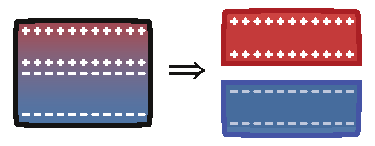
\includegraphics[width=0.55\textwidth]{images/chp7/chp7assenzamonopoli1.pdf}
\end{center}
Un \textbf{dipolo magnetico}\index{dipolo!magnetico}, invece, si separa sempre in altri dipoli! Ad esempio, se un magnete a barra viene tagliato a metà, non si avrà una metà con il polo nord e l'altra con il polo sud, ma \textit{ciascun pezzo} avrà un suo polo nord e polo sud.
\begin{center}
	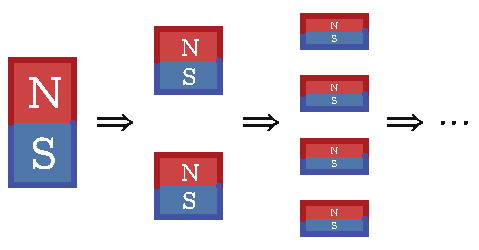
\includegraphics[width=0.55\textwidth]{images/chp7/chp7assenzamonopoli2.pdf}
\end{center}
\begin{observe}
	Per analogia con il dipolo elettrico, si usa indicare il \textit{polo nord} di un magnete con il segno $+$ e il \textit{polo sud} con il segno $-$.
\end{observe}
\paragraph{Le linee di forza}
Se ad oggi parliamo di campi vettoriali nell'elettromagnetismo, probabilmente parte del merito lo dobbiamo allo scienziato inglese \textbf{Michael Faraday} (1791 - 1867). Durante i suoi esperimenti sul magnetismo, circa intorno al 1831, egli notò la maniera peculiare con cui della \textit{limatura di ferro} si disponeva su un cartoncino o una lastra di vetro in presenza di un magnete: essa sembrava disporsi naturalmente lungo delle \textit{linee} che si estendevano da un \textit{polo} all'altro del magnete. Faraday ipotizzò quindi che i magneti esercitava delle forze lungo queste ``linee di forza'', che secondo Faraday dovevano esistere in qualche modo \textit{fisicamente}.
\begin{center}
	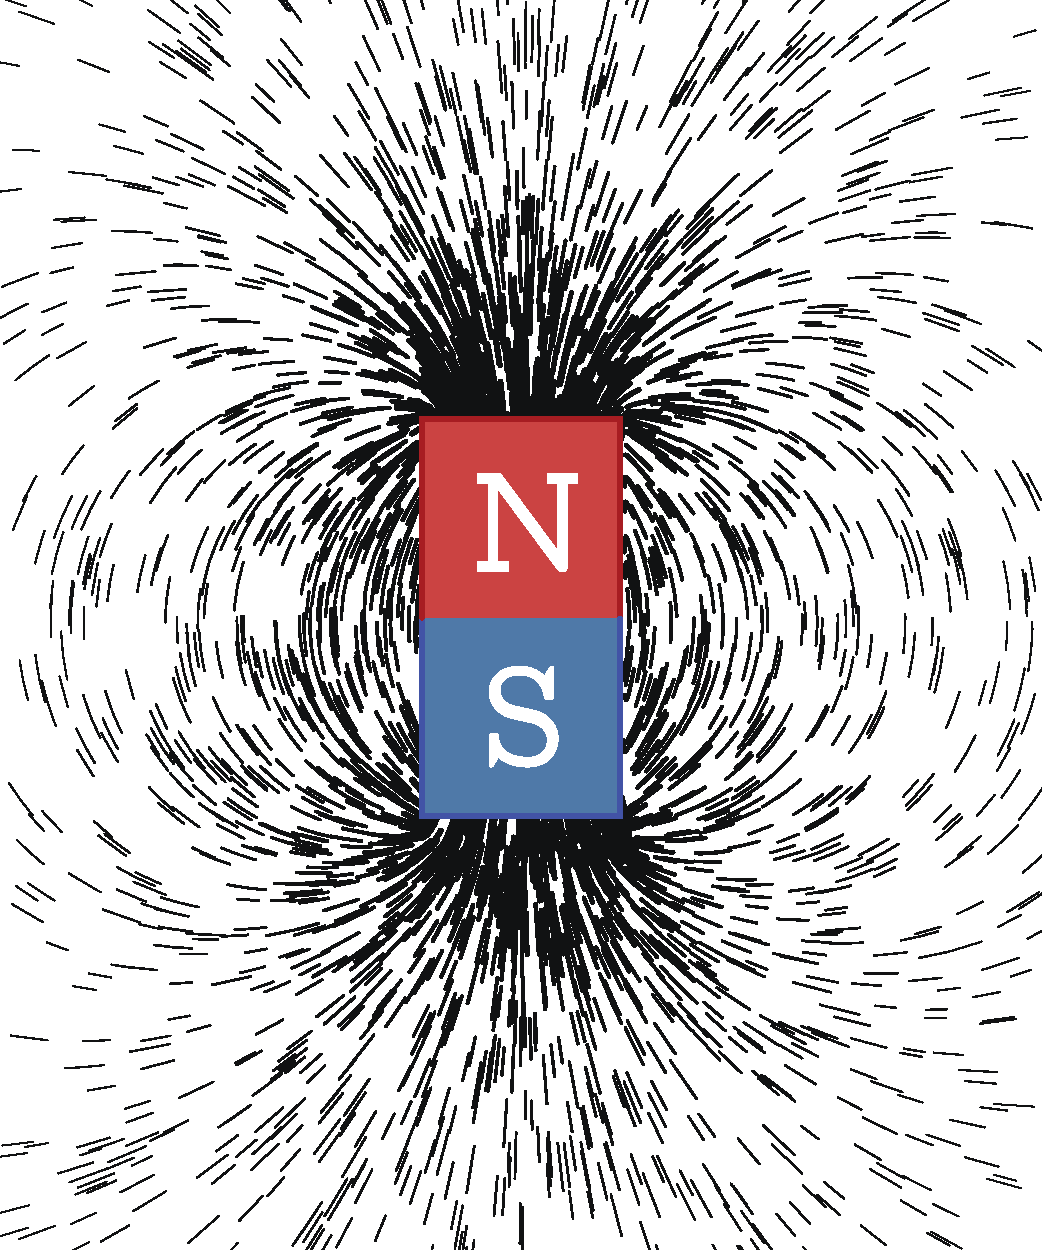
\includegraphics[width=0.3\textwidth]{images/chp7/chp7faradayfilatura.pdf}
\end{center}
Le osservazioni di Faraday anticipano la descrizione moderna dei fenomeni magnetici: come è stato per quelli elettrici, la descrizione del magnetismo passa per il \textit{formalismo dei campi vettoriali}: in questo caso, le forze sono l'applicazione in un punto del \textbf{campo magnetico}\index{campo!magnetico} $\vba{B}$ generato, ad esempio, da magneti; le linee di forza sono, ovviamente, le curve tali per cui in ogni loro punto il vettore tangente alla curva è il vettore dato da $\vba{B}$.
\section{Legge di Gauss per la magnetostatica}
Le linee di campo svolgono un ruolo fondamentale per capire la prima, grossa differenza tra il campo magnetico e quello elettrico: il flusso attraverso una superficie chiusa.\\
Analizziamo la questione dal punto di vista matematico, confrontandola con una situazione a noi \textit{famigliare}. Ricordiamo che, nel \textit{dipolo elettrico}, le linee di campo si sviluppano come in figura.
\begin{center}
	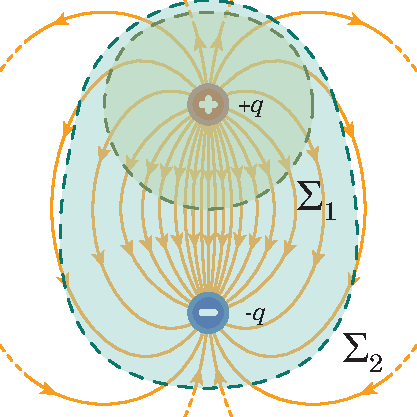
\includegraphics[width=0.35\textwidth]{images/chp7/chp7leggegaussmagneti1.pdf}
\end{center}
Prese due superfici $\Sigma_1$ e $\Sigma_2$, la prima contenente la \textit{carica positiva} e la seconda \textit{entrambe}, si ha
\begin{equation*}
	\Phi_{\Sigma_1}(\vba{G})=\frac{q}{\epsilon_0}\qquad\Phi_{\Sigma_2}(\vba{E})=\frac{q-q}{\epsilon_0}=0
\end{equation*}
Con un dipolo magnetico ci ritroviamo una situazione simile.
\begin{center}
	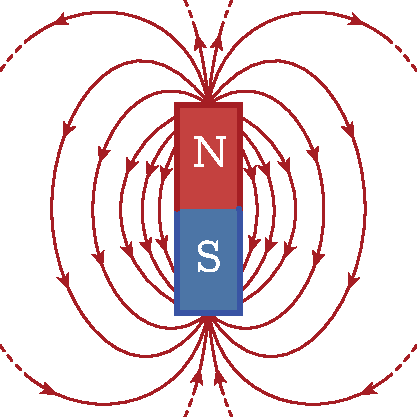
\includegraphics[width=0.35\textwidth]{images/chp7/chp7leggegaussmagneti2.pdf}
\end{center}
Come osservò Faraday con la limatura di ferro, le linee di forza che visualizziamo \textit{attorno} al magnete sono uguali a quelle \textit{esterne} del dipolo elettrico. Ci possiamo però chiedere cosa succedere all'\textit{interno} del magnete. Se proviamo a spezzare a metà il magnete, si creano delle linee di forze ``interne'' tra i due magnetini ma, a differenza del dipolo elettrico, sono rivolte verso l'alto e non verso il basso - di fatto, sembra che le linee di forza delle curve orientate chiuse!
\begin{center}
	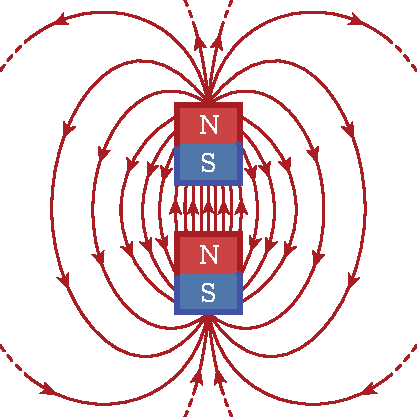
\includegraphics[width=0.35\textwidth]{images/chp7/chp7leggegaussmagneti3.pdf}
\end{center}
Se continuiamo a \textit{dividere} i magneti, le linee di forza che si vengono a formare tra di essi continuano ad essere in tale maniera. Pertanto, dobbiamo aspettarci che le linee di forza all'esterno proseguano all'interno e formino delle \textit{curve orientate chiuse}.
\begin{center}
	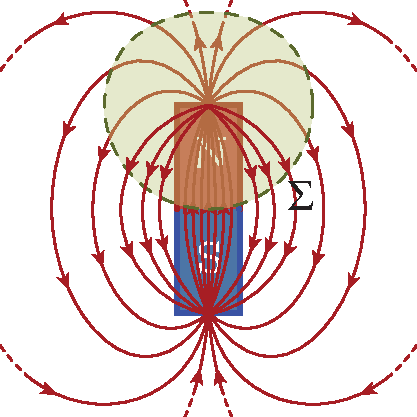
\includegraphics[width=0.35\textwidth]{images/chp7/chp7leggegaussmagneti4.pdf}
\end{center}
Osserviamo che la forza di interazione magnetostatica di Coulomb è inversamente proporzionale a $r^2$, pertanto potremmo applicare una versione ``magnetica'' della legge di Gauss\footnote{In modo analogo a come abbiamo fatto nell'osservazione a pag. \pageref{LeggeGaussMoltoGeneralizzata}, \autoref{chap:FlussoCampoElettrico}.}. Tuttavia, per quanto osservato sperimentalmente, non sappiamo costruire o produrre dei \textit{monopoli magnetici}, pertanto dobbiamo sempre considerare un dipolo magnetico.
Si noti che, se applichiamo la legge di Gauss ad una superficie contenente un \textit{dipolo elettrico}, il flusso sarà nullo. La situazione è analoga per il caso magnetico: non possiamo individuare dei monopoli, certo, ma dal polo nord esce un numero di linee di flusso pari a quelle che entrano dal polo sud - non può esistere una ``carica magnetica'' totale differente da zero. Di conseguenza, abbiamo mostrato empiricamente la
\begin{theorema}[Legge di Gauss per la magnetostatica]\index{legge!di Gauss!per la magnetostatica}
	Il flusso del campo magnetostatico $\vba{B}$ attraverso un superficie \textbf{chiusa} è nullo.
	\begin{itemize}
		\item \textbf{Forma integrale:}
		\begin{equation}
			\tcboxmath[colback=yellowpastellow!30!white,colframe=redsalsa!85!black,drop fuzzy shadow, nobeforeafter, math upper, tcbox raise base, enhanced]{\Phi_\Sigma(\vba{B})=\int_{\Sigma}\vba{B}\vdot \vbh{u}_nd\Sigma=0}\label{LeggeGaussMagnetismoIntegrale}
		\end{equation}
		\item \textbf{Forma differenziale:}
		\begin{equation}
			\tcboxmath[colback=yellowpastellow!30!white,colframe=redsalsa!85!black,drop fuzzy shadow, nobeforeafter, math upper, tcbox raise base, enhanced]{\div{\vba{B}}=0}\label{LeggeGaussMagnetismoDifferenziale}
		\end{equation}
	\end{itemize}
\end{theorema}
\begin{demonstration}
	Deriviamo la forma differenziale. Per il teorema della divergenza si ha
	\begin{equation*}
		0=\Phi_\Sigma(\vba{B})=\int_{\Sigma}\vba{B}\vdot \vbh{u}_nd\Sigma=\int_V\div{\vba{B}}
	\end{equation*}
	dove $V$ è il volume racchiuso da $\Sigma$, ossia $\partial V=\Sigma$. Poichè tale relazione è vera per ogni volume $V$, si ha l'uguaglianza delle integrande:
	\begin{equation*}
		\div{\vba{B}}=0\qedhere
	\end{equation*}
\end{demonstration}
Tale legge è una delle due \textit{equazioni di Maxwell per la magnetostatica}.

Una conseguenza immediata della legge di Gauss per il magnetismo è che il campo magnetostatico è un \textbf{campo solenoidale}\footnote{Nella ``Raccolta Differenziata'', a pag. \ref{CampoSolenoidale} è possibile trovare la definizione di campo solenoidale e altre proprietà.}, a differenza del campo elettrostatico che è \textit{conservativo}.
\begin{digression}
	Se, in futuro, si dovessero scoprire i monopoli magnetici, la legge di Gauss per il magnetismo sarebbe del tutto analoga a quella per l'elettricità: il flusso del campo magnetico $\vba{B}$ attraverso una superficie chiusa è proporzionale alla \textit{carica magnetica} in essa racchiusa o, in forma differenziale, la divergenza di $\vba{B}$ è proporzionale ad un'apposita \textit{densità di carica magnetica} $\rho_m$. La forma originale della legge di Gauss si avrebbe soltanto in presenza di una densità di carica magnetica \textit{nulla}.
\end{digression}
\section{Interazioni con le cariche in moto}
Come si è potuto notare, gli studi dei fenomeni magnetici erano inizialmente separati da quell sull'elettricità, dato che i due fenomeni risultavano scorrelati. Ed effettivamente con le nostre conoscenze moderne sappiamo perché: le leggi che descrivono i fenomeni \textit{magnetostatici} sono \textit{indipendenti} da aspetti di natura \textit{elettrica}. Purtuttavia, per diversi secoli aleggiò il sospetto che ci fosse un legame tra elettricità e magnetismo, ma per avere dei risultati concreti si dovette aspettare gli studi con la \textit{corrente elettrica}.
\subsection{L'esperimento di Oersted}\index{esperimento!di Oersted}
Il primo ad identificare un legame tra l'elettricità e il magnetismo fu il fisico danese \textbf{Hans Christian Oersted} (1777-1851), che il 21 Luglio 1820 pubblicò le sue scoperte in un libricino di quattro pagine scritto in latino.\\
Qualche mese prima, il 21 Aprile 1820, nel preparare una lezione serale all'Università di Copenhagen, Oersted notò che la corrente in un filo spostava (seppur molto debolmente) l'ago di una bussola ad posta lì vicino.
Per studiare meglio tale effetto, Oestred costruì un apparato apposito: preso un filo nella direzione nord-sud, fissò sotto di esso un ago di bussola, parallelo ad esso. Facendo passare un'intensitò di corrente elevata, notò che l'ago tendeva a \textit{deviare} la propria direzione allontanandosi dal nord magnetico, a cui normalmente puntava, per porsi \textit{perpendicolarmente} al filo. Inoltre, notò che:\\
\begin{minipage}{0.3\textwidth}
	\begin{center}
		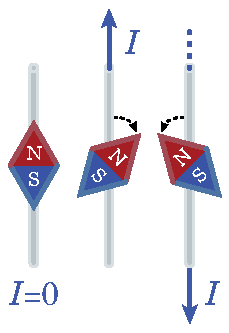
\includegraphics[width=1\textwidth]{images/chp7/chp7oersted1.pdf}
	\end{center}
\end{minipage}\hspace{5pt}
\begin{minipage}{0.69\textwidth}
	\begin{itemize}
		\item La \textit{deflessione} era inversamente proporzionale alla \textit{distanza} dell'ago dal filo.
		\item Se il filo veniva posto sotto l'ago, invece che sopra, l'ago si muoveva nella direzione \textit{opposta}; la stessa cosa accadeva invertendo la direzione della corrente, ma mantenendo fissa la posizione della bussola.
		\item La deflessione non dipendeva dal materiale del filo.
		\item Una deflessione avveniva anche in presenza di materiali come legno, vetro, resina, metalli e acqua tra l'ago e il filo.
	\end{itemize}
\end{minipage}\\
Pur non avendo alcun idea del \textit{perché}\footnote{Oestred cercò di spiegarlo come la conseguenza di un ``\textit{conflictus electricus}'' (\textit{conflitto elettrico}), il cui significato è da ritrovarsi nella filosofia di Oerstred e di conseguenza tralasceremo bellamente in quanto del tutto irrilevante ai nostri scopi.}, il fisico danese concluse che la ``\textit{forza magnetica}'', che in termini moderni interpretiamo come \textit{campo magnetico}, doveva soddisfare le seguenti proprietà:\\
\begin{minipage}{0.69\textwidth}
	\begin{itemize}
		\item Le linee di campo magnetico circondando il filo in cui passa la corrente, formando delle circonferenze.
		\item Le linee di campo magnetico sono situate su un \textit{piano perpendicolare al filo}. In altre parole, il campo magnetico non ha componenti lungo il filo ed è tangente alle circonferenze.
		\item Se la direzione della corrente è invertita, il verso della forza è invertita.
		\item Il campo magnetico generato dal filo non dipende dal suo materiale.
		%\item Il campo magnetico si può osservare anche in presenza di certe sostanze.
	\end{itemize}
\end{minipage}\hspace{5pt}
\begin{minipage}{0.3\textwidth}
	\begin{center}
		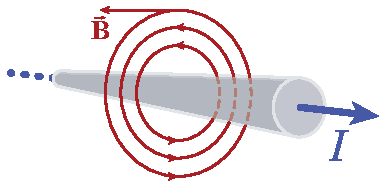
\includegraphics[width=1\textwidth]{images/chp7/chp7oersted2.pdf}
	\end{center}
\end{minipage}
\begin{digression}
	Ancor più di scoprire che la corrente agisse su un ago magnetico, fu una sorpresa considerevole per gli scienziati dell'epoca il fatto che la direzione della ``\textit{forza magnetica}'' (in termini moderni, del campo magnetico) fosse \textit{perpendicolare} ad un piano passante per il filo e l'ago.\\
	Infatti, dato che la \textit{legge di Coulomb} delle interazioni dei corpi carichi e dei corpi magnetizzati alla fine non era altro che una variante della \textit{legge di gravitazione universale di Newton}, la quale afferma che l'attrazione gravitazionale agisce lungo le linee che collegano i corpi massivi, ci si aspettava che valesse una legge simile anche per le interazioni tra un corpo percorso da corrente e un corpo magnetico.
\end{digression}
\subsection{L'esperimento di Ampère}\index{esperimento!di Ampère}\label{EsperimentodiAmpere}
Anche il francese \textbf{Andre Marie Ampère} (1775-1836), che abbiamo incontrato in precedenza nel trattare la corrente elettrica, propose un esperimento analogo nel 1823.\\
Ampère osservò che due fili paralleli nei quali le corrente scorre nella \textit{stessa direzione} sono \textit{attratti} tra di loro, mentre se la corrente è percorsa in \textit{senso opposto} i fili tendono ad \textit{allontanarsi}. In entrambi i casi, la forza su un filo è \textit{uguale e contraria} a quella esercitata sull'altro.\\
\begin{minipage}{0.49\textwidth}
	\begin{center}
		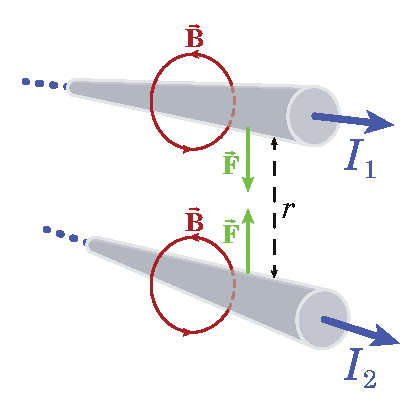
\includegraphics[width=1\textwidth]{images/chp7/chp7ampere1.pdf}
	\end{center}
\end{minipage}
\begin{minipage}{0.49\textwidth}
	\begin{center}
		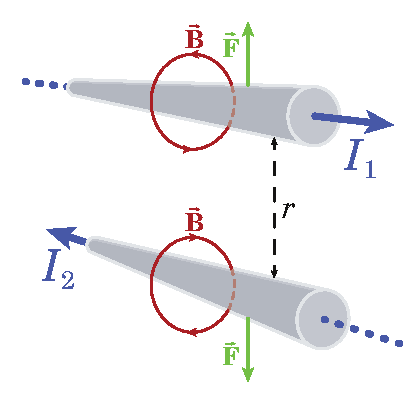
\includegraphics[width=1\textwidth]{images/chp7/chp7ampere2.pdf}
	\end{center}
\end{minipage}\\
Sperimentalmente, si trovò che la \textit{densità lineare} di forza era descritta dalla \textbf{legge (della forza) di Ampère}\index{legge! della forza di Ampère}
\begin{equation}
	\tcboxmath[colback=yellowpastellow!30!white,drop fuzzy shadow, nobeforeafter, math upper, tcbox raise base, enhanced]{\frac{F}{\mathcal{l}}=k\frac{I_1I_2}{r}}
\end{equation}
dove $\mathcal{l}$ è la lunghezza dei fili, $r$ la distanza tra i due e $I_1$, $I_2$ le correnti che scorrono in essi e $k$ un'opportuna costante; nel sistema SI si pone pari a
\begin{equation}
	\tcboxmath[colback=yellowpastellow!30!white,drop fuzzy shadow, nobeforeafter, math upper, tcbox raise base, enhanced]{k=\frac{\mu}{4\pi}=\SI[per-mode = fraction]{d-7}{\newton\per\ampere\squared}}
\end{equation}
dove $\mu_0$ è detta \textbf{permeabilità magnetica del vuoto}\index{costante!di permeabilità magnetica!del vuoto} ed è definita esattamente come
\begin{equation}
	\tcboxmath[colback=yellowpastellow!30!white,drop fuzzy shadow, nobeforeafter, math upper, tcbox raise base, enhanced]{\mu_0=4\pi\cdot\SI[per-mode = fraction]{d-7}{\newton\per\ampere\squared}}
\end{equation}
È facile immaginare che nell'esperimento di Ampère le correnti fungono da ``cariche magnetiche''. La legge che descrive tale fenomeno è quindi l'equivalente per la magnetostatica della \textit{legge di Coulomb per l'elettrostatica}.
\paragraph{Una (obsoleta) definizione dell'ampere}
Nel \autoref{chap:correnteElettrica} abbiamo parlato dell'\textit{ampere}, l'unica unità fondamentale che introdurremo in questo testo. Dato che è una delle unità base da cui poter derivare tutte le altre, dobbiamo chiaramente \textit{definirlo}.\\
La prima definizione dell'ampere pre-SI - detto ``\textit{Ampere Internazionale}'' - era definito elettro-chimicamente come la corrente necessaria per depositare $\SI{1.118}{\milli\gram}$ di argento al secondo da una soluzione di nitrato d'argento. Nel 1939 si propose una definizione migliore - ma tecnicamente diversa, dato che fra le due unità c'era una differenza del $0.015\%$ - che utilizzava proprio l'esperimento di Ampère:
\begin{define}[Ampere {(1960)}]
	L'\textbf{ampere}\index{ampere} è quella corrente costante che, se mantenuta in due conduttori paralleli rettilinei, di lunghezza infinita e sezione circolare trascurabile, posti a un metro l'uno dall'altro nel vuoto, produce tra questi una forza pari a $\SI{2d-7}{\newton}$ per ogni metro di lunghezza.
\end{define}
La conseguenza di tale definizione fu che la permeabilità magnetica del vuoto era una \textit{costante} ben precisa, pari a
\begin{equation*}
	\mu_0=4\pi\cdot\SI[per-mode = fraction]{d-7}{\newton\per\ampere\squared}
\end{equation*}
...o almeno, questo era vero fino al 2019. Dalla sua introduzione nel 1960 fino a tale anno, il SI era basato su sette \textit{unità base}, su cui le altre derivano. Per quanto coerente ed efficace, erano evidenti alcuni problemi:
\begin{itemize}
	\item il chilogrammo era ancora pari al peso del campione fisico del 1889 depositato al \textit{Ufficio internazionale dei pesi e delle misure}, il quale era però prono a piccoli ma rilevanti variazioni nell'arco degli anni - considerati inaccettabili per la crescente precisione richiesta negli esperimenti.
	\item Altre unità, come il kelvin e l'ampere, erano basati su misure difficilmente realizzabili con precisione in un laboratorio. 
\end{itemize}
Si decise quindi di cambiare il focus: il sistema non partiva direttamente dalle sette unità in sè, bensì avrebbe fissato con estrema precisione il valore di sette \textit{costanti fondamentali}, da cui poter ricavare la misura delle unità di base e poi delle derivate in modo consistente e ripetibile in laboratorio. Per tale motivo, quattro delle sette unità fondamentali - il chilogrammo, il kelvin, la mole e, ultimo ma non per importanza, l'ampere - vennero ridefinite. L'ampere, nello specifico, venne definito fissando il valore in ampere per secondo (ossia in coulomb) della carica elementare:
\begin{define}[Ampere {(2019)}]
	L'\textbf{ampere}\index{ampere}, simbolo $A$, è l'unità del SI della corrente elettrica. È definito considerando il valore numerico costante della carica elementare pari a $1.602176634\cdot10^{-19}$ quando espresso nell'unità $\unit{\coulomb}$, che equivale a $\unit{\ampere\second}$, dove il secondo è definito in termini di $\Delta \nu_{\textrm{Cs}}$.\footnote{Dove $\Delta \nu_{\textrm{Cs}}$ è il valore fissato della frequenza della radiazione emessa dall'atomo di Cesio 133 nella transizione tra due livelli iperfini (F=4, M=0) e (F=3, M=0) dello stato fondamentale $~^2(1/2)$.'' Parole complesse per dire sostanzialmente che anche il secondo $\unit{\second}$ è basato su una costante fisica definita.} 
\end{define}
Una conseguenza di ciò è che la permeabilità magnetica del vuoto non è più fissata esattamente, ma deve essere ricavata sperimentalmente - anche se il valore di $4\pi\cdot\SI[per-mode = fraction]{d-7}{\newton\per\ampere\squared}$ è una buona approssimazione per i calcoli più teorici. In questo testo considereremo la situazione pre-2019, anche solo per una mera questione di semplificazione dei calcoli.
\section{La forza di Lorentz}
Dagli esperimenti di Oersted e Ampère sappiamo che si devono necessariamente considerare gli effetti della corrente elettrica nello studio del magnetismo; tuttavia, ci manca ancora una descrizione \textit{qualitativa} delle leggi che descrivono ciò.

All'inizio, si ipotizzò che la forza che agiva in questi fenomeni dovesse essere dipendente dalla \textit{distanza} tra gli oggetti, ma tale approccio si rivelò inconclusivo. Fu solo dopo la \textit{teoria delle linee di forza} di Faraday e la loro descrizione matematica da parte di \textbf{Lord Kelvin} (1850-1925) e \textbf{James Clark Maxwell} (1831-1879) che si parlò di tale forza in termini di campo elettrico e magnetico.\\
Nonostante con gli occhi moderni una formulazione differenziale di tale forza è già visibile nelle famose equazioni di Maxwell, al tempo di Maxwell non era evidente come tali leggi fossero collegate con le forze che muovono gli oggetti carichi. La legge che vediamo fu prima formulata da \textbf{J. J. Thomson} (1824-1907), sebbene con un fattore errato a causa di qualche errore di calcolo, derivandola dalle leggi di Maxwell; fu poi nel 1895 l'olandese \textbf{Hendrik Lorentz} (1853-1928) a derivare  - tramite il formalismo vettoriale introdotto da \textbf{Oliver Heaviside} (1850-1925) - la legge che tuttora porta il suo nome\footnote{Nulla da togliere a Lorentz, ma J. J. Thomson  fece buona parte del lavoro. Almeno un ringraziamento poteva concederglielo, suvvia.}.
\begin{define}[Forza di Lorentz]
	La \textbf{forza di Lorentz}\index{forza!di Lorentz} $\vba{F}$ esercitata su una carica elettrica $q$ in movimento con velocità $\vba{v}$, in un certo punto e ad un certo istante, dal campo elettrico $\vba{E}$ e dal campo magnetico $\vba{B}$ è
	\begin{equation}
		\tcboxmath[colback=yellowpastellow!30!white,colframe=ceruleancrayola!85!black,drop fuzzy shadow, nobeforeafter, math upper, tcbox raise base, enhanced]{\vba{F}_L=q\left(\vba{E}+\vba{v}\cross\vba{B}\right)}
	\end{equation}
\end{define}
Spesso si parla di forza di Lorentz anche per indicare la sola componente della forza elettromagnetica che è legata al campo magnetico, ossia
\begin{equation}
		\tcboxmath[colback=yellowpastellow!30!white,drop fuzzy shadow, nobeforeafter, math upper, tcbox raise base, enhanced]{\vba{F}_L=q\vba{v}\cross\vba{B}}
\end{equation}
\begin{center}
	\begin{minipage}{0.49\textwidth}
		\begin{center}
			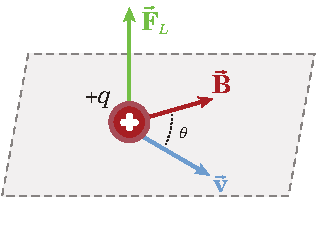
\includegraphics[width=1\textwidth]{images/chp7/chp7forzalorentz1.pdf}
		\end{center}
	\end{minipage}
	\begin{minipage}{0.49\textwidth}
		\begin{center}
			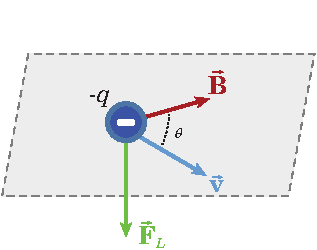
\includegraphics[width=1\textwidth]{images/chp7/chp7forzalorentz2.pdf}
		\end{center}
	\end{minipage}
\end{center}
Da qui in poi ci riferiremo, se non specificato diversamente, a questa seconda interpretazione della \textit{legge di Lorentz}.
\paragraph{Il lavoro della forza di Lorentz}
Il lavoro della forza di Lorentz è nullo. Infatti,
\begin{equation}
	W=\int \vba{F}_L\vdot d\vba{s}=\int q\vba{v}\cross\vba{B}\vdot d\vba{s}=0
\end{equation}
dato che lo spostamento infinitesimo è \textit{parallelo} alla velocità della particella e quindi il prodotto scalare risulta nullo. Di conseguenza, la variazione di energia cinetica è nulla.
\begin{equation*}
	W=\Delta E_k=\frac{1}{2}mv_{f}^2-\frac{1}{2}mv_{i}^2=0\implies{v_1}^2={v_f}^2
\end{equation*}
La forza di Lorentz \textit{non} modifica il modulo della velocità della particella.
\subsection{La forza di Lorentz con campo magnetico uniforme: il caso perpendicolare alla velocità}
Essendo un prodotto vettoriale, nel caso di un campo magnetico uniforme $\vba{B}$ si ha la forza massima se $\vba{v}$ è perpendicolare al campo - in tal caso il modulo della forza è
\begin{equation*}
	F=qvB
\end{equation*}
La direzione è data dalla \textit{regola della mano destra}, mentre il verso dipende dal segno di $q$.
\begin{observe}
	Un campo magnetico uniforme \textit{non} produce un'accelerazione tangenziale, ma solo una \textit{centripeta} per l'ortogonalità di $\vba{F}$ rispetto alla velocità $\vba{v}$. Il moto è quindi \textit{circolare uniforme}. 
\end{observe}
\paragraph{Raggio di curvatura}
Da
\begin{equation*}
	\vba{F}_L=m\vba{a}\implies q\vba{v}\cross\vba{B}=m\vba{a},
\end{equation*}
noto che $\vba{a}$ è solo quella centripeta, si ha
\begin{equation*}
	q\Ccancel[red]{v}B=ma_C=m\frac{v^{\Ccancel[red]{2}}}{r}
\end{equation*}
da cui segue l'espressione del \textbf{raggio di curvatura}:
\begin{equation}
	\tcboxmath[colback=yellowpastellow!30!white,drop fuzzy shadow, nobeforeafter, math upper, tcbox raise base, enhanced]{r=\frac{mv}{qB}}
\end{equation}
Il raggio di curvatura è inversamente proporzionale all'intensità del campo e alla carica, mentre è direttamente proporzionale alla quantità di moto.
\paragraph{Velocità angolare}
La velocità angolare è, in modulo,
\begin{equation}
	\omega=\frac{v}{r}=\frac{qB}{m}
\end{equation}
mentre vettorialmente è
\begin{equation}
	\tcboxmath[colback=yellowpastellow!30!white,drop fuzzy shadow, nobeforeafter, math upper, tcbox raise base, enhanced]{\vba{\omega}=-\frac{q\vba{B}}{m}}
\end{equation}
dato che $\vba{v}=\vba{r}\cross\vba{\omega}$.
\paragraph{Periodo del moto}
Il periodo del moto è
\begin{equation}
	\tcboxmath[colback=yellowpastellow!30!white,drop fuzzy shadow, nobeforeafter, math upper, tcbox raise base, enhanced]{T=\frac{2\pi}{\omega}=\frac{2\pi m}{qB}}
\end{equation}
\subsection{La forza di Lorentz con campo magnetico uniforme: il caso generale}
In generale, il modulo della forza di Lorentz risulta
\begin{equation*}
	F_L=qvB\sin\theta=q v_n B
\end{equation*}
dove $\theta$ è l'angolo compresa tra la velocità $v$ e il campo $\vba{B}$. Se consideriamo l'asse $z$ allineato con il campo $\vba{B}$, la velocità della particella può essere scissa in due: la velocità normale $v_n$ e la velocità $v_z$ parallela all'asse $z$.\\
La forza di Lorentz influenza la velocità normale e non quella parallela. Perpendicolarmente al campo $\vba{B}$, la particella è nella stessa situazione studiata nella sezione precedente: in particolare, la particella subisce un'accelerazione centripeta con moto circolare uniforme, il cui raggio di curvatura è
\begin{equation}
	\tcboxmath[colback=yellowpastellow!30!white,drop fuzzy shadow, nobeforeafter, math upper, tcbox raise base, enhanced]{r=\frac{mv_n}{qB}=\frac{mv\sin\theta}{qB}}
\end{equation}
Lungo l'asse $z$, la velocità $v_z$ risulta costante. Il moto descritto dalla particella è complessivamente un \textit{moto elicoidale}, la cui accelerazione costante è perpendicolare sia alla velocità $\vba{v}$, sia al campo magnetico $\vba{B}$.\\
\paragraph{Passo dell'elica}
\begin{define}[Passo dell'elica]
	Il \textbf{passo} di un moto elicoidale\index{passo di un'elica}  è lo spazio percorso dalla particella lungo l'asse dell'elica dopo un avvolgimento completo, ossia dopo un periodo:
	\begin{equation}
		\tcboxmath[colback=yellowpastellow!30!white,colframe=ceruleancrayola!85!black,drop fuzzy shadow, nobeforeafter, math upper, tcbox raise base, enhanced]{p=v_zT}
	\end{equation}
\end{define}
Nel caso dell'elica dovuta alla forza di Lorentz:
\begin{equation}
	p=v_zT=\frac{2\pi}{qB}v_z=\frac{2\pi}{qB}v\cos\theta
\end{equation}
\subsection{Applicazioni della forza di Lorentz}
\paragraph{Bottiglia magnetica}
\begin{define}[Bottiglia magnetica]
	Una \textbf{bottiglia magnetica}\index{bottiglia magnetica} è una configurazione particolare del campo magnetico in cui l'intensità del campo cambia muovendosi parallelamente: ai lati e negli estremi della bottiglia c'è un campo magnetico molto più intenso della parte centrale.
\end{define}
Se una particella entra nel campo magnetico della bottiglia, può succedere che la particella venga intrappolata all'interno della bottiglia. Infatti, la particella subisce ai lati una forza di Lorentz così intensa da far cambiare direzione alla velocità.
\begin{center}
	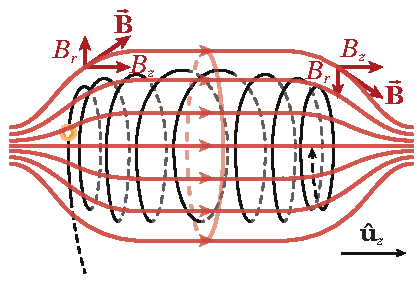
\includegraphics[width=0.45\textwidth]{images/chp7/chp7bottigliamagnetica1.pdf}
\end{center}
\begin{example}[Fascia di Van Allen]
	Nel campo magnetico terrestre - più di preciso nella \textit{magnetosfera} che circonda la Terra - ci sono due zone toroidali, dette \textbf{fasce di Van Allen}\footnote{Da non confondere con le \textit{fasce di van Halen}, accessori del chitarrista olandese Eddie van Halen.}, che fungono da bottiglie magnetiche per le particelle cariche che si spostano nello spazio.
	\begin{center}
		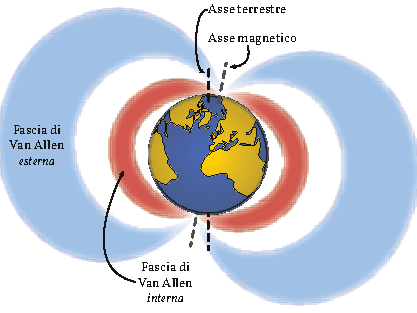
\includegraphics[width=0.55\textwidth]{images/chp7/chp7vanallen.pdf}
	\end{center}
	Nella fascia di Van Allen \textit{interna}, il campo magnetico è particolarmente elevato e contiene alte concentrazioni di elettroni e protoni, con energia rispettivamente nell'ordine delle centinaia di $\unit{\kilo\electronvolt}$ e maggiori di $\SI{100}{\mega\electronvolt}$.\\
	Nella fascia di Van Allen \textit{esterna}, il campo magnetico è più debole e contiene principalmente elettroni ad alta energia (tra $0,1$ e $\SI{100}{\mega\electronvolt}$).
\end{example}
\paragraph{Spettrometro di massa}
\begin{define}[Spettrometro di massa]
	Uno \textbf{spettrometro di massa}\index{spettrometro di massa} è uno strumento che, avvalendosi di campi elettrici e magnetici, permette di misurare la massa di particelle atomiche.
\end{define}
Nel tipico spettrometro di massa una sorgente, ad esempio di ioni, emette delle particelle in un campo elettrico dovuto a delle armature. Esse vengono quindi accelerate dal campo elettrico lì presente, per poi entrare in un campo magnetico uniforme uscente dal piano in cui le particelle si muovono: esse vengono deflesse dal campo e, curvando la loro traiettoria, colpiscono un rilevatore di velocità.
	\begin{center}
	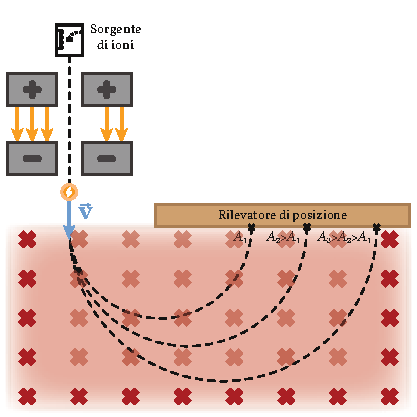
\includegraphics[width=0.45\textwidth]{images/chp7/chp7spettrometro.pdf}
\end{center}
Tra la fine delle armature e l'inizio del campo magnetico, l'energia cinetica della particella è dovuta esclusivamente dall'energia potenziale fornita dal campo:
\begin{equation*}
	E_C=E_P\implies \frac{1}{2}mv^2=qV\implies v=\sqrt{\frac{2qV}{m}}
\end{equation*}
Qui $V$ è il potenziale del campo elettrico. Il raggio di curvatura del campo magnetico diventa allora
\begin{equation*}
	r=\frac{mv}{qB}=\sqrt{\frac{2mV}{q}}\frac{1}{B}
\end{equation*}
ed è evidente che particelle con egual carica ma massa diversa avranno raggi di curvatura diversa.\\
In particolare, lo spettrometro è utilizzato per distinguere la massa degli \textbf{isotopi}\index{isotopo} di uno stesso elemento chimico, ossia atomi che presentano lo stesso \textit{numero atomico} (ugual numero di \textit{protoni} e di \textit{elettroni} rispetto l'atomo standard), ma diversa massa atomica a causa di un numero differente di \textit{neutroni}.
Se $A_1$ e $A_2$ sono le masse atomiche di tali isotopi, allora
\begin{equation*}
	\frac{A_1}{A_2}=\frac{r_1^2}{r_2^2}
\end{equation*}
misurando la posizione sul rilevatore ci permette quindi di distinguere la massa e di rapportarle tra di loro.
\paragraph{Effetto Hall}
Consideriamo un conduttore, ad esempio a forma di parallelepipedo, messo in un campo magnetico diretto verso $x$.
\begin{center}
	\begin{minipage}{0.49\textwidth}
		\begin{center}
			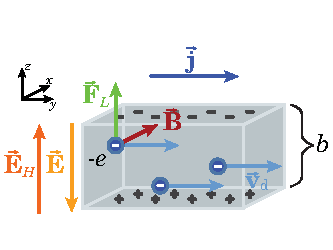
\includegraphics[width=1\textwidth]{images/chp7/chp7effettohall1.pdf}
		\end{center}
	\end{minipage}
	\begin{minipage}{0.49\textwidth}
		\begin{center}
			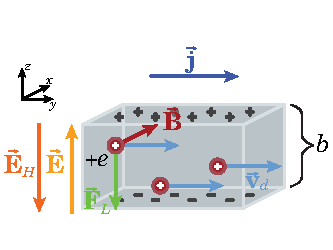
\includegraphics[width=1\textwidth]{images/chp7/chp7effettohall2.pdf}
		\end{center}
	\end{minipage}
\end{center}
In esso, le cariche si muovono con una certa velocità di deriva $\vba{v}_d$, dove
\begin{equation*}
	\vba{j}=ne\vba{v}_d
\end{equation*}
\begin{itemize}
	\item Se a muoversi sono le cariche \textit{positive}, si pone $e>0$.
	\item Se a muoversi sono le cariche \textit{negative}, si pone $e<0$.
\end{itemize}
Il campo magnetico esercita su ciascuna delle particelle in moto nel conduttore una \textit{forza di Lorentz}
\begin{equation*}
	\vba{F}_L=e\vba{v}_d\cross\vba{B}
\end{equation*}
che, per la regola della mano destra, ha direzione l'asse $z$ e verso dipendente dal segno della carica:
\begin{itemize}
	\item se $e>0$, $\vba{F}_L$ va verso l'alto.
	\item se $e<0$, $\vba{F}_L$ va verso il basso.
\end{itemize}
Si verifica quindi una separazione di cariche positive e negative, creando una differenza di potenziale e di conseguenza un campo elettrico all'interno del conduttore, che chiameremo \textbf{campo di Hall}\index{campo!di Hall} in onore del suo scopritore \textbf{Edwin Hall} (1855-1938).
\begin{equation}
	\tcboxmath[colback=yellowpastellow!30!white,drop fuzzy shadow, nobeforeafter, math upper, tcbox raise base, enhanced]{\vba{E}_H=\frac{\vba{F}_L}{e}=\vba{v}_d\cross\vba{B}=\frac{\vba{j}}{ne}\cross\vba{B}}
\end{equation}
Quando le cariche si separano si viene a formare una nuova situazione di equilibrio: il campo elettrico  $\vba{E}_H$ causato dal campo magnetico deve essere compensato da un campo uguale ed opposto, che per separazione di cariche è dato da
\begin{equation}
	\vba{E}=-\vba{E}_H=\Delta V b\vbh{z}
\end{equation}
dove $b$ è l'altezza del parallelepipedo. La presenza di un campo magnetico crea una \ddp tra le due pareti del conduttore.
\begin{equation*}
	\Delta V=\int \vba{E}_H\vdot d\vba{z}=\pm vBb
\end{equation*}
Il valore di $\vba{E}_H$ \textit{non} dipende quindi dalla carica in sé (e quindi da $\vba{j}$), ma dalla sua velocità. Invece, ciò che dipende dai portatori di carica è il segno, dato che dipende dalla direzione verso della corrente e quindi dalla carica:
\begin{itemize}
	\item Se le cariche sono \textit{positive}, il segno è positivo.
	\item Se le cariche sono \textit{negative}, il segno è negativo.
\end{itemize}
È dunque possibile distinguere, in due conduttori con stessa corrente $\vba{j}$, se i portatori di carica sono positivi e negativi misurando il segno del potenziale, il quale dipende esclusivamente dal segno delle cariche.
\begin{example}
	Grazie all'effetto Hall si è potuto osservare che nei \textit{conduttori metallici} la carica che si muove è \textit{negativa}.
\end{example}
\begin{digression}
	Per la natura stessa dell'atomo, è molto più facile avere elettroni liberi - e quindi cariche negative che si spostano - rispetto ad avere nuclei liberi da elettroni (o addirittura protoni!) e quindi carica positiva che si sposta.\\
	Ciò non significa che non capita mai di avere corrente portata da cariche positive: capita in certi tipi di \textit{semiconduttori}, ma la spiegazione di tali moti si riconduce ai \textit{moti di lacune}, la cui spiegazione rientra in quei meandri della \textit{meccanica quantistica} che - per nostra fortuna - non approfondiremo. 
\end{digression}

\paragraph{Selettore di velocità}
Consideriamo la situazione in figura: due piastre cariche creano un campo elettrico $\vba{E}$ tra di esse; al contempo è presente tra le armature un campo magnetico uniforme $\vba{B}$ perpendicolare al campo elettrico.
\begin{center}
	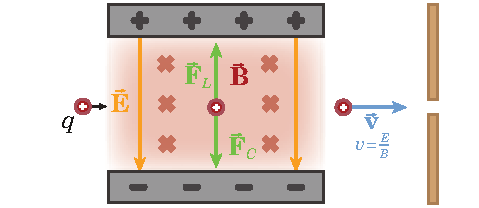
\includegraphics[width=0.45\textwidth]{images/chp7/chp7selettore.pdf}
\end{center}
Prendiamo un fascio di particelle di carica $q$ che entrano dentro le piastre con velocità $\vba{v}$ perpendicolare sia al campo elettrico, sia al campo magnetico: esse sono soggette sia alla \textit{forza di Lorentz} $\vba{F}_L$ in quanto particelle in movimento, ma sono soggette anche ad un \textit{forza di Coulomb} $\vba{F}_C$ data dal campo magnetico delle piastre.
\begin{align*}
	F_L=qvB&&F_C=qE
\end{align*}
Alla fine del conduttore prendiamo una parete con una sottilissima apertura che fa passare solo le particelle non deviate, cioè tali per cui la loro velocità sia tale da equilibrare le due forze.
\begin{equation*}
	F_L=F_C\implies \Ccancel[red]{q}vB=\Ccancel[red]{q}E
\end{equation*}
\begin{equation}
	\tcboxmath[colback=yellowpastellow!30!white,drop fuzzy shadow, nobeforeafter, math upper, tcbox raise base, enhanced]{v=\frac{E}{B}}
\end{equation}
Cambiando l'intensità del campo elettrico $\vba{E}$ e del campo magnetico $\vba{B}$ è possibile selezionare solo le particelle che hanno velocità data dal rapporto dei due campi.
\subsection{Unità di misura del campo magnetico}
Dalla forza di Lorentz si definisce l'unità di misura del campo magnetico, il \textbf{tesla}\index{tesla}.
\begin{equation*}
	\left[B\right]=\frac{[F]}{[q][V]}=\frac{\unit[per-mode = fraction]{\newton}}{\unit{\coulomb}\unit[per-mode = fraction]{ \meter\per\second}}=\unit[per-mode = fraction]{\kilogram\per\coulomb\per\second} = \unit[per-mode = fraction]{\kilogram\per\ampere\per\second\squared}
\end{equation*}
\begin{units}~\\
	\textbf{\textsc{Campo magnetico:}} tesla ($\unit{\tesla}$).\\
	\textit{\textbf{Dimensioni:}} $[\vba{B}]=\dfrac{[F]}{[q][V]}=\mathsf{M} \mathsf{T}^{-2}  \mathsf{I}^{-1}$
\end{units}
	\begin{examples}~
		\begin{itemize}
			\item Il campo magnetico terrestre è dell'ordine di $\SI[exponent-product=\ensuremath{\cdot}]{d-5}{\tesla}$.
			\item Il campo magnetico di un tipico magnete da frigo è di $\SI[exponent-product=\ensuremath{\cdot}]{5d-3}{\tesla}$.
			\item Il campo magnetico sulla superficie di un magnete al neodimio è di $\SI[exponent-product=\ensuremath{\cdot}]{1.25}{\tesla}$.
			\item Il campo magnetico all'interno del \textit{Large Hadron Collider} al \textit{CERN} è $\SI[exponent-product=\ensuremath{\cdot}]{8}{\tesla}$.
			\item Il campo magnetico più forte mai realizzato da un magnete fu di  $\SI[exponent-product=\ensuremath{\cdot}]{97.4}{\tesla}$.
		\end{itemize}
	\end{examples}
Come molte altre unità che abbiamo incontrato, i tesla sono ordini di grandezza \textit{molto più elevati} rispetto ai campi magnetici che si usano sperimentalmente; per questo si fa spesso uso dei \textit{sottomultipli} del tesla, come ad esempio il \textbf{gauss}\index{gauss (unità di misura)} ($\text{G}$), pari a
\begin{equation}
	\SI[exponent-product=\ensuremath{\cdot}]{1}{\text{G}}=\SI[exponent-product=\ensuremath{\cdot}]{d-4}{\tesla}
\end{equation}
\section{Seconda legge di Laplace}
La \textit{forza di Lorentz} ci permette di quantificare l'interazione tra una particella in movimento e il campo magnetico. Per quanto sia un importantissimo risultato teorico e abbia anche delle immediate applicazioni pratiche - ad esempio per spiegare il funzionamento dei tubi a raggi catodici - ha un problema: generalmente non studiamo singole cariche in movimento, bensì un numero estremamente elevato sotto forma di \textit{corrente elettrica}. La \textbf{seconda legge di Laplace}, che descrive l'interazione magnetica dovuta ad una corrente elettrica costante, fu inizialmente scoperta \textit{ancor prima} della forza di Lorentz con metodi \textit{sperimentali}; noi invece la deriveremo in via teorica con la suddetta forza di Lorentz.
\begin{theorema}[Seconda legge di Laplace]\index{legge!di Laplace!seconda}
	La \textbf{forza di Laplace}\index{forza!di Laplace} è la forza magnetica esercitata da un campo magnetico $\vba{B}$ su un filo $\gamma$ di parametrizzazione $\vba{r}$ percorso da corrente. Essa è pari a
	\begin{align}
		\tcboxmath[colback=yellowpastellow!30!white,colframe=redsalsa!85!black,drop fuzzy shadow, nobeforeafter, math upper, tcbox raise base, enhanced]{\vba{F}=\int_{\gamma} I d\vba{s}\cross\vba{B}\qquad\text{dove}\qquad d\vba{s}=\dv{\vba{r}(t)}{t}dt}
	\end{align}
dove $d\vba{s}$ segue la direzione della corrente nel filo.
\end{theorema}
\begin{demonstration}
	Ricordiamo che la corrente elettrica che attraversa una porzione di filo è
	\begin{equation*}
		\vba{j}=ne\vba{v}_d=jd\vba{s}
	\end{equation*}
	dove $n$ è il numero di cariche per unità di volume e $\vba{v}_d$ la velocità di deriva; l'ultima eguaglianza è dovuta al fatto ch per un conduttore filiforme come quello in esame $d\vba{s}$ si può orientare come $\vba{j}$. Su ogni singola carica $e$ la forza di Lorentz \textit{media} sarebbe
	\begin{equation*}
		\vba{F}_L=e\vba{v}_d\cross\vba{B}
	\end{equation*}
	Un tratto infinitesimo di conduttore avente lunghezza $ds$ e sezione $\Sigma$ ha volume $\Sigma ds$ e contiene $n$ elettroni; segue che la forza agente per unità di volume infinitesimo è
	\begin{equation*}
		\frac{d\vba{F}}{dV}=ne\vba{v}_d\cross\vba{B}=\vba{j}\cross\vba{B}
	\end{equation*}
	Complessivamente, su un filo di volume $V$ (che possiamo considerare di sezione costante $\Sigma$) si ha
	\begin{equation}
		\vba{F}=\int_V\vba{j}\cross\vba{B}dV=\int_{\gamma} jd\vba{s}\cross\vba{B}\underbrace{\int_{\Sigma}d\Sigma}_{=\Sigma}=\int_{\gamma} j\Sigma d\vba{s}\cross\vba{B}\squarequal
	\end{equation}
	Ricordando che l'intensità di corrente nel filo è definita come il flusso di corrente
	\begin{equation*}
		I=\Phi_{\Sigma}\left(\vba{j}\right)=j\Sigma
	\end{equation*}
	si ha
	\begin{equation*}
		\squarequal\int_{\gamma} Id\vba{s}\cross\vba{B}\qedhere
	\end{equation*}
\end{demonstration}
\begin{example}\label{RisultateSpiraNulla}
	Supponiamo di avere un campo magnetico uniforme in cui è immerso un filo con corrente stazionaria. Dato che si può portar fuori dall'integrale sia la corrente sia il campo magnetico, allora si ha
	\begin{equation}
		\vba{F}=I\int d\vba{s}\cross\vba{B}=I\left(\vba{r}_2-\vba{r}_1\right)\cross\vba{B}
	\end{equation}
In particolare, se il circuito è chiuso, vale
\begin{equation}
	\vba{F}=I\oint d\vba{s}\cross\vba{B}=0
\end{equation}
\end{example}
\begin{examplewt}[Bilancia magnetica]
	Consideriamo un lungo circuito percorso da corrente $I$ posto su un piano verticale. Una sua parte a forma di ferro di cavallo come in figura, di larghezza $\mathcal{l}$, è immersa in un campo magnetico uniforme $\vba{B}$ uscente dal piano.
	\begin{center}
		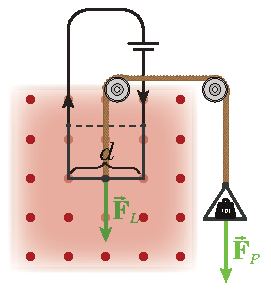
\includegraphics[width=0.45\textwidth]{images/chp7/chp7bilanciamagnetica.pdf}
	\end{center}
	Se il valore della corrente $I$ e della larghezza $d$ è noto, posso misurare la forza di Laplace utilizzando una bilancia: all'equilibrio, la forza di Laplace ha lo stesso valore della forza peso.\\
	Inoltre, è possibile calcolare il modulo del \textit{campo magnetico}: se le forze all'equilibrio sono
	\begin{equation*}
		\begin{cases}
			F_L=I\mathcal{l}B\\
			F_P=mg
		\end{cases}
	\end{equation*}
	allora, imponendo l'uguaglianza tra di esse, si ha
	\begin{equation*}
		B=\frac{mg}{I\mathcal{l}}
	\end{equation*}
\end{examplewt}
\section{Il momento meccanico di un circuito piano in un campo magnetico}\label{spirarettangolaremeccanica}
Consideriamo una \textbf{spira}\index{spira} - un circuito chiuso, in sostanza - rettangolare di lati $a$ e $b$ percorsa da una corrente (in modulo) $I$, immersa in un campo magnetico $\vba{B}$ uniforme. Chiamiamo $\theta$ l'angolo compreso tra $\vba{B}$ e il versore normale $\vbh{u}_n$ alla superficie racchiusa dalla spira; il verso di $\vbh{u}_n$ è dettato da una \textit{variante} della \textit{regola della mano destra}.\\
Data una curva orientata, il verso del versore normale $\vbh{u}_n$ alla superficie delimitata da tale curva è definito nella seguente maniera: curvando le dita della mano in modo che le dita della mano seguano l'orientazione della curva - nel nostro caso, seguendo la corrente che percorre la spira - il pollice retto punta nel verso di $\vbh{u}_n$.\\
Le forze magnetiche $\vba{F}_3$ e $\vba{F}_4$ sui lati \textit{orizzontali} sono uguali e contrarie e hanno la stessa retta di azione, dato che sono applicate nel centro del lato./
\begin{center}
	\begin{minipage}{0.49\textwidth}
		\begin{center}
			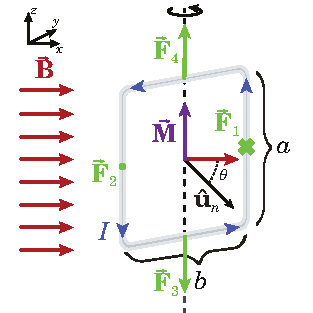
\includegraphics[width=1\textwidth]{images/chp7/chp7momentospira1.pdf}
		\end{center}
	\begin{center}
		{\scriptsize Vista di 3/4.}
	\end{center}
	\end{minipage}
	\begin{minipage}{0.49\textwidth}
		\begin{center}
			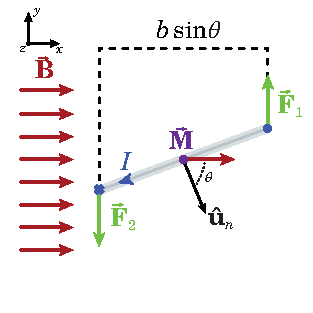
\includegraphics[width=1\textwidth]{images/chp7/chp7momentospira2.pdf}
		\end{center}
		\begin{center}
		{\scriptsize Vista dall'alto.}
		\end{center}
	\end{minipage}
\end{center}
Una situazione simile si verifica con le forze $\vba{F}_{1}$ e $\vba{F}_2$ sui lati \textit{verticali}: le forze sono uguali e contrarie, di valore massimo $IaB$. Infatti,
	\begin{equation*}
		\abs{\vba{F}}=I\abs{\int_{lato\ verticale} d\vba{s}}\abs{\vba{B}}=IaB
	\end{equation*}
in quanto $\abs{\int_{lato\ verticale} d\vba{s}}=a$ e $\vba{B}$ è ortogonale ai lati. Di conseguenza, sulla spira la risultante delle forze è nulla e non si ha un \textit{movimento traslatorio}.\\
Tuttavia, c'è una differenza sostanziale dal primo caso: la coppia di forze laterali \textit{non} hanno la stessa retta di azione! Come si può facilmente vedere guardando la spira dall'alto, tale coppia di forze generano sulla spira un \textit{momento di coppia} attorno all'asse verticale del centro di massa e dunque una \textit{rotazione}.

\begin{attention}
	Il \textit{momento di una forza} e il \textit{momento di una coppia di forze} sono strettamente correlati ma hanno differenze fondamentali.
	\begin{itemize}
		\item Il \textbf{momento $\vba{M}$ di una forza} $\vba{F}$ rispetto ad un punto $O$ è definito come il prodotto vettoriale tra la forza $\vba{F}$ e il vettore distanza tra $O$ e il punto di applicazione di $\vba{F}$.
		\begin{equation}
			\tcboxmath[colback=yellowpastellow!30!white,colframe=darkdarkred!85!black,drop fuzzy shadow, nobeforeafter, math upper, tcbox raise base, enhanced]{\vba{M}=\vba{r}\cross\vba{F}}
		\end{equation}
		Esso \textit{dipende} dal punto $O$, cambia se cambiamo il punto $O$ ed è l'equivalente rotazionale di una forza lineare nel caso in cui l'oggetto a cui la forza è applicata sia libero di ruotare attorno ad un perno.
		\item Il \textbf{momento $\vba{M}$ di una \emph{coppia} di forze}\footnote{In alcuni testi lo si distingue dal momento di una forza $\vba{M}$ usando la nomenclatura $\vba{\tau}$; noi, ahimè, per adeguarci ad una convenzione malsana non faremo ciò.} $\vba{F}$ e $-\vba{F}$ è definito come il prodotto vettoriale tra il vettore distanza $\vba{d}$  tra i punti di applicazione delle forze e $\vba{F}$
		\begin{equation}
			\tcboxmath[colback=yellowpastellow!30!white,colframe=darkdarkred!85!black,drop fuzzy shadow, nobeforeafter, math upper, tcbox raise base, enhanced]{\vba{M}=\vba{d}\cross\vba{F}}
		\end{equation}
Esso \textit{non} dipende da alcun punto di riferimento, a differenza del momento di una forza, ed è pertanto un vettore ``libero''. Il momento di una coppia di forze è la \textit{somma vettoriale} dei momenti di ciascuna forza rispetto ad un punto scelto $O$; di conseguenza, è un caso \textit{particolare} del momento di una forza.\\
Si può generalizzare il momento di coppia se abbiamo un sistema di più forze la cui risultante è nulla.
	\end{itemize}
\end{attention}
Calcoliamo tale momento di coppia. Possiamo calcolarlo in due modi: come somma dei momenti delle singole forze o come momento di una coppia. Sebbene sia nettamente più rapido procedere con il secondo metodo, per completezza\footnote{Ma soprattutto perché è il metodo presentato per qualche motivo non ben specificato durante il corso.} presentiamo anche il primo.
\begin{itemize}
	\item \textbf{Somma dei momenti.} Consideriamo come punto di applicazione il centro della spira: le distanze $\vba{r}_i$ dal centro ai punti di applicazione delle forze $\vba{F}_i$ sono uguali ed opposte, con modulo $\frac{b}{2}$. Segue quindi che il momento di coppia ha modulo pari a due volte il momento di una delle forze (ad esempio, a $\vba{M}_1=\vba{r}_1\cross\vba{F}_1=\vba{r}\cross\vba{F}$). Notiamo che tra $\vba{F}$ e $\vba{r}$ c'è, per ragioni geometriche, un angolo pari a $\theta$; denotata la direzione del momento con il versore $\vbh{u}_M$, si ha
	\begin{align*}
		\vba{M}&=\vba{r}_1\cross \vba{F}_1+\vba{r}_2\cross \vba{F}_2=2\vba{r}\cross\vba{F}=2\abs{\vba{r}}\abs{\vba{F}}\sin\theta\vbh{u}_M=\\
		&=2\frac{b}{2}IaB\sin\theta\vbh{u}_M=Iab B \sin\theta\vbh{u}_M=\\
		&=I\Sigma B\sin\theta\vbh{u}_M
	\end{align*}
dove $\Sigma=ab$ è l'area della spira.
\item \textbf{Momento di coppia.} La distanza vettoriale $\vba{d}$ tra i punti di applicazione ha modulo pari a $b$ e si noti che, per ragioni geometriche, l'angolo tra $\vba{d}$ e una delle forze $\vba{F}$ è $\theta$. Si ha
	\begin{equation*}
	\vba{M}=\vba{d}\cross\vba{F}=\abs{\vba{d}}\abs{\vba{F}}B \sin\theta\vbh{u}_M=Iab B \sin\theta\vbh{u}_M=I\Sigma B\sin\theta\vbh{u}_M
\end{equation*}
\end{itemize}
Si noti che il versore $\vbh{u}_M$ è ottenibile anche come prodotto vettoriale (normalizzato!) di $\vba{B}$ con $\vbh{u}_n$:
\begin{equation}
	\vbh{u}_M=\frac{\vbh{u}_n\cross\vba{B}}{\abs{\vbh{u}_n\cross\vba{B}}}=\frac{\vbh{u}_n\cross\vba{B}}{B\sin\theta}
\end{equation}
Riscriviamo $\vba{M}$ con questo prodotto vettoriale:
\begin{equation*}
	\vba{M}=I\Ccancel[red]{B}\Sigma\Ccancel[red]{\sin\theta}\frac{\vbh{u}_n\cross\vba{B}}{\Ccancel[red]{B}\Ccancel[red]{\sin\theta}}=I\Sigma\vbh{u}_n\cross\vba{B}
\end{equation*}
Introduciamo ora la seguente definizione.
\begin{define}[Momento magnetico della spira]
	Data una spira di area $\Sigma$ percorsa da una corrente $I$, chiamiamo il \textbf{momento magnetico della spira}\index{momento!magnetico di una spira} la quantità vettoriale
	\begin{equation}
		\tcboxmath[colback=yellowpastellow!30!white,colframe=ceruleancrayola!85!black,drop fuzzy shadow, nobeforeafter, math upper, tcbox raise base, enhanced]{\vba{m}=I\Sigma\vbh{u}_n}
	\end{equation}
\end{define}
Otteniamo che il momento meccanico della spira rettangolare è
\begin{equation}
	\tcboxmath[colback=yellowpastellow!30!white,drop fuzzy shadow, nobeforeafter, math upper, tcbox raise base, enhanced]{\vba{M}=\vba{m}\cross\vba{B}}
\end{equation}
\subsection{Il caso generale}
Nel caso di una spira generica immersa in un campo magnetico uniforme sappiamo già che la risultante delle forze è nulla\footnote{Si veda l'esempio a pag. \pageref{RisultateSpiraNulla}.}, quindi non abbiamo alcun moto traslatorio. Tuttavia, a meno di casi specifici, c'è un momento meccanico - il cui punto di applicazione è arbitrario, che porta ad una rotazione della spira.
\begin{theorema}[Momento meccanico di una spira]
	Una spira generica, da intendersi come un circuito piano chiuso di area $\Sigma$, percorsa da corrente costante $I$ e immersa in un campo magnetico uniforme $\vba{B}$ subisce un momento meccanico pari a
	\begin{equation}
		\tcboxmath[colback=yellowpastellow!30!white,colframe=redsalsa!85!black,drop fuzzy shadow, nobeforeafter, math upper, tcbox raise base, enhanced]{\vba{M}=\vba{m}\cross\vba{B}}
	\end{equation}
	dove
	\begin{equation}
		\tcboxmath[colback=yellowpastellow!30!white,colframe=redsalsa!85!black,drop fuzzy shadow, nobeforeafter, math upper, tcbox raise base, enhanced]{\vba{m}=I\Sigma\vbh{u}_n}
	\end{equation}
	è il \textit{momento magnetico} associato ad essa.
\end{theorema}
\begin{comment}
	\begin{observe}
		Nelle ``XXX'', a pag. \pageref{XXX} è possibile trovare una dimostrazione alternativa più ``fisica'', basata sui risultati ottenuti con la spira rettangolare.
	\end{observe}
\end{comment}
\begin{demonstration}
	Dato che in questo contesto abbiamo a che fare con un corpo continuo, il momento deve essere formulato per mezzo di un \textit{integrale}. Fissato un punto di riferimento arbitrario da cui misurare il vettore posizione $\vba{r}$, se
	\begin{equation*}
		d\vba{F}=Id\vba{s}\cross \vba{B}
	\end{equation*}
	è la forza per unità di lunghezza, il momento meccanico per unità di lunghezza è
	\begin{equation*}
		d\vba{M}=I\vba{r}\cross d\vba{F}
	\end{equation*}
	Il momento meccanico complessivo si ottiene integrando lungo $\gamma$:
	\begin{equation*}
		\vba{M}=\oint_\gamma d\vba{M}=\oint_\gamma \vba{r}\cross d\vba{F}=I \oint_\gamma \vba{r}\cross\left(d\vba{s}\cross\vba{B}\right)
	\end{equation*}
		Poniamo come parametrizzazione della curva $\gamma$ la funzione $\vba{r}=\vba{r}(t)$ nell'intervallo $\left[t_1, t_2\right]$, $\vba{r}(t_1)=\vba{r}(t_2)$. Ricordiamo che lo spostamento infinitesimo è
	\begin{equation*}
		d\vba{s}=\dv{\vba{r}}{t}dt=\vbd{r}dt
	\end{equation*}
	Segue che
	\begin{equation*}
		\vba{M}=I\oint_\gamma \vba{r}\cross\left(d\vba{s}\cross\vba{B}\right)=I\int_{t_1}^{t_2}\vba{r}\cross\left(\vbd{r}\cross\vba{B}\right)dt\squarequal
	\end{equation*}
	Ricordiamo l'\textit{identità di Jacobi} del prodotto vettoriale
	\begin{equation*}
		\vba{r}\cross\left(\vbd{r}\cross\vba{B}\right)+\vba{B}\cross\left(\vba{r}\cross\vbd{r}\right)+\vbd{r}\cross\left(\vba{B}\cross\vba{r}\right)=0
	\end{equation*}
	All'ultimo termine applichiamo la regola di Leibniz al contrario:
	\begin{align*}
		\vbd{r}\cross\left(\vba{B}\cross\vba{r}\right)&=\dv{t}\left(\vba{r}\cross\left(\vba{B}\cross\vba{r}\right)\right)-\vba{r}\cross\dv{t}\left(\vba{B}\cross\vba{r}\right)=\\
		&=\dv{t}\left(\vba{r}\cross\left(\vba{B}\cross\vba{r}\right)\right)-\vba{r}\cross\left(\vba{B}\cross \vbd{r}\right)=\\
		&=\dv{t}\left(\vba{r}\cross\left(\vba{B}\cross\vba{r}\right)\right)+\vba{r}\cross\left(\vbd{r}\cross\vba{B}\right)
	\end{align*}
	Sostituendo nell'identità di Jacobi, otteniamo
	\begin{equation*}
		2\vba{r}\cross\left(\vbd{r}\cross\vba{B}\right)+\vba{B}\cross\left(\vba{r}\cross\vbd{r}\right)+\dv{t}\left(\vba{r}\cross\left(\vba{B}\cross\vba{r}\right)\right)=0
	\end{equation*}
	da cui
	\begin{align*}
		\squarequal& -\frac{I}{2}\int_{t_1}^{t_2}\left[\dv{t}\left(\vba{r}\cross\left(\vba{B}\cross\vbd{r}\right)\right)+\vba{B}\cross\left(\vba{r}\cross\vbd{r}\right)\right]dt\\
		=&\frac{I}{2}\underbrace{\eval{\vba{r}\cross\left(\vba{B}\cross\vbd{r}\right)}_{t_1}^{t_2}}_{=0\ \circled{\ast}}+\frac{I}{2}\int_{t_1}^{t_2}\left(\vba{r}\cross\vbd{r}\right)\cross\vba{B}dt=\frac{I}{2}\left(\int_{t_1}^{t_2}\vba{r}\cross\vbd{r}dt\right)\cross\vba{B}\squarequal
	\end{align*}
	dove si ha l'uguaglianza $\quad\circled{\ast}\quad$ in quanto la spira è chiusa e il valore di tale quantità è la stessa sia in $t_1$, sia in  $t_2$.\\
	Possiamo dimostrare\footnote{Nelle ``Note aggiuntive'', a pag. \pageref{AreaCurvaDelimitata}, è possibile trovare tale dimostrazione.} che
	\begin{equation*}
		\Sigma\vbh{u}_n=\frac{1}{2}\int_{t_1}^{t_2}\vba{r}\cross\vbd{r}dt
	\end{equation*}
pertanto,
\begin{equation*}
	\squarequal I\Sigma\vbh{u}_n\cross \vba{B}=\vba{m}\cross\vba{B}\qedhere
\end{equation*}
\end{demonstration}
\paragraph{Condizione di equilibrio}
Dato che il momento risultante è ottenibile come un prodotto vettoriale tra il momento magnetico $\vba{m}$ e il campo magnetico $\vba{B}$, la spira risulta essere in equilibrio se $\vba{m}$ è parallelo a $\vba{B}$. Se $\theta$ è l'angolo tra il campo e la normale alla spira, allora
\begin{itemize}
	\item $\theta = 0$: equilibrio stabile.
	\item $\theta = \pi$ equilibrio instabile.
\end{itemize}
Consideriamo un asse di rotazione parallelo a $\vba{M}$ e sia $\mathbf{I}$ il momento d'inerzia della spira attorno a tale asse. Ricordiamo che il \textit{momento angolare} si può esprimere in funzione dell'\textit{accelerazione angolare}:
\begin{equation}
	M=\mathbf{I}\alpha=\mathbf{I}\dv[2]{\theta}{t}
\end{equation}
Per piccole oscillazioni, si ha che $\sin\theta\sim\theta$ e quindi
\begin{equation*}
	-\mathbf{I}\Sigma B\theta=\mathbf{I}\dv[2]{\theta}{t}
\end{equation*}
\begin{equation}
	\tcboxmath[colback=yellowpastellow!30!white,drop fuzzy shadow, nobeforeafter, math upper, tcbox raise base, enhanced]{\dv[2]{\theta}{t}+\omega^2\theta=0\quad\text{dove}\quad\omega^2=\frac{I\Sigma B}{\mathbf{I}}=\frac{m B}{\mathbf{I}}}
\end{equation}
Il comportamento delle piccole oscillazioni ricorda quello di un \textit{oscillatore armonico}.
\paragraph{Energia potenziale}
L'energia potenziale del moto angolare è
\begin{equation}
	\tcboxmath[colback=yellowpastellow!30!white,drop fuzzy shadow, nobeforeafter, math upper, tcbox raise base, enhanced]{U_P=-\vba{m}\vdot\vba{B}=-I\Sigma B\cos\theta}
\end{equation}
Allora
\begin{equation}
	\tcboxmath[colback=yellowpastellow!30!white,drop fuzzy shadow, nobeforeafter, math upper, tcbox raise base, enhanced]{\abs{\vba{M}}=\dv{U_P}{\theta}=I\Sigma B\sin\theta}
\end{equation}\label{EnergiaPotenzialeCasoGeneralemanontroppo}
\begin{center}
	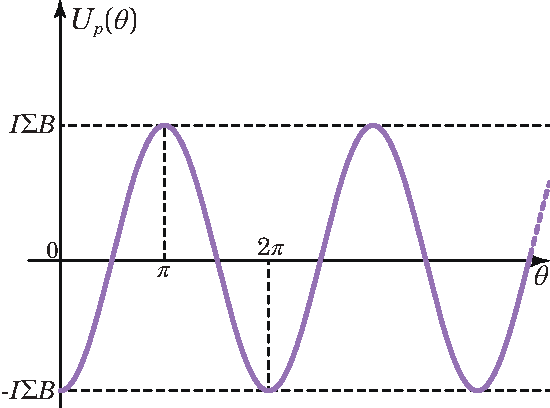
\includegraphics[width=0.75\textwidth]{images/chp7/chp7graficoenergiapot.pdf}
\end{center}
\paragraph{Il principio di equivalenza di Ampère}\label{principio di equivalenza di ampere}
Si può osservare come un \textit{ago magnetico} immerso in un campo magnetico si comporta, per piccole oscillazioni, in \textit{modo analogo} a quanto visto con la spira percorsa da corrente - ma un ago magnetico non è altro che un dipolo magnetico! Ciò ci porta ad affermare quello che chiamiamo \textbf{principio di equivalenza di Ampere}.
\begin{principle}[Principio di equivalenza di Ampère]\index{principio!di equivalenza di Ampère}
	Un circuito elettrico piano di area $d\Sigma$ percorso da una corrente $I$ è equivalente ad un dipolo elementare in termini di campo magnetico generato e degli effetti meccanici causati da un campo magnetico \textit{esterno}. Il dipolo equivalente ha momento magnetico
	\begin{equation}
		\tcboxmath[colback=yellowpastellow!30!white,colframe=CGblue!85!black,drop fuzzy shadow, nobeforeafter, math upper, tcbox raise base, enhanced]{d\vba{m}=Id\Sigma \vbh{u}_n}
	\end{equation}
	perpendicolare al piano della spira e orientata rispetto al verso della corrente secondo la \textit{regola della vite}.
\end{principle}
Chiaramente, parlando di un'equivalenza il ragionamento è bilaterale: ogni qual volta incontreremo un dipolo magnetico possiamo immaginarlo come se fosse una spira percorsa corrente.
